\chapter[Particle Identification and Event Reconstruction]{Particle Identification and Event Reconstruction}
\label{chap:ParticleID}




\section{Particle Flow}
\label{sec:PF}

The Particle Flow (PF) algorithm \cite{CMS-PAS-PFT-09-001} identifies and reconstructs all the stable-visible particles produced in the hard interaction, by
combining the information collected by the CMS sub-detectors in order to optimize the determination of their direction, energy and type. The PF 
technique performs the global event reconstruction classifying all the visible particles into five mutually exclusive groups: photons, 
neutral hadrons, charged hadrons, electrons and muons. This list of individual particles (called ``PF Candidates'') are used 
as an input in further algorithms to reconstruct higher level objects such as jets, missing transverse energy and tau-leptons. \\

%The capabilities of the CMS detector are ideal for using the PF technique as a global event reconstruction. The high 
%granularity of the inner tracker and the ECAL, the hermiticity of the HCAL, the high performance of the muon system 
%along with the strong magnetic field provided by the superconducting solenoid allow PF technique to reach a 
%high performance reconstruction for the individual particles produced in the hard interaction, even for charged particles
%with very low $\textrm{p}_{\textrm{T}}$ of an order of 100 MeV; this leads to an improvement in the energy jet corrections. Besides, the high performance of the individual particle reconstruction 
%allows to discriminate between nearby tracks such as the decay products of the tau-lepton. The main advantage 
%to use the PF technique as a global event reconstruction is the high performance reconstruction 
%for all the physics objects, in particular jets, MET and tau-leptons \cite{CMS-PAS-PFT-10-001}.\\


The capabilities of the CMS detector are ideal for using the PF technique as a global event reconstruction. The high 
granularity of the inner tracker and the ECAL, the hermiticity of the HCAL, the high performance of the muon system 
along with the strong magnetic field provided by the superconducting solenoid allow PF technique to reach a 
high performance reconstruction for the individual particles produced in the hard interaction, even for charged particles
with very low $\textrm{p}_{\textrm{T}}$ (of the order of 100 MeV). This leads to an improvement in the global event 
reconstruction since, instead of using special sub-detectors designed to reconstruct an specific 
object (like alternative event reconstruction techniques), PF algorithm uses a more completed information collected 
by all CMS sub-detectors, avoiding any ambiguity to reconstruct the object. Besides, the 
individual particle reconstruction provides a detailed information 
about compositeness of high level objects like jets, allowing PF technique
to determinate the hadron profile of the jet and its origin, which is important for the tau-identification. 
Additionally, the high performance of individual particle reconstruction allows to discriminate between nearby tracks 
such as the decay products of the tau-lepton. The main advantage 
to use the PF technique as a global event reconstruction is the high performance reconstruction 
for all the physics objects, in particular jets, MET and tau-leptons \cite{CMS-PAS-PFT-10-001}.\\

%and the ECAL, the hermicity of the HCand clusters with high efficiency.

The PF technique is performed in three steps: First, the algorithm builds the so-called ``PF elements'' which consist of tracks 
reconstructed in the Inner Tracker, energy clusters reconstructed in the calorimeters and tracks observed in the muon system;
the second stage addresses the topological association of the basic PF elements each other using the ``link-algorithm''; finally,
individual particles are identified and reconstructed from the content of the linked elements. \\

%Photons are reconstructed from its energy deposits in the ECAL (See section \ref{sec:Photon});
%electrons are reconstructed by the combination of tracks and the energy deposits in the ECAL of the electron itself and the 
%Brestrahlung radiation produced by its interaction with the tracker material (See section \ref{sec:Electron}); Muon reconstruction 
%is performed connecting together the tracks reconstructed by the inner tracker and the muon system, it will be described in section \ref{sec:Muon};

\subsection{Track Reconstruction}
\label{subsec:TrackReco}
The track reconstruction in the inner tracker is one of the most important keys of the global event reconstruction. The inner tracker, due to its
high granularity, provides a precise reconstruction of the charged-particle tracks and consequently give rise to an accurate reconstruction 
of the primary vertex, identifying it from the pileup interactions. \\

The track reconstruction is performed in several steps by a process called \textit{iterative tracking}. In the initial iterations, 
the iterative tracking applies a tight criteria in order to search for tracks easy to identify (tracks 
with relative high $\textrm{p}_{\textrm{T}}$ produced near the interaction region). In the next iterations, the hits 
unambiguously assigned to a track are removed. This reduces the combinatorial complexity in the subsequent iterations 
and allows to loosen the selection criteria to identify the tracks associated with low $\textrm{p}_{\textrm{T}}$. In the first three iterations, 
the iterative tracking reaches an efficiency up to 99.5$\%$ for isolated muons and larger than 90$\%$ for 
charged hadrons in jets \cite{CMS-PAS-PFT-09-001}. Last iterations relaxes the constrains on the origin of the vertex 
to find tracks originated outside the beam spot (secondary charged particles from photon conversions in the tracker material) 
and to reconstruct the remaining tracks. Each iteration could be summarized in 4 steps:\\

\begin{itemize}
 \item Tracks are seeded using 2 or 3 hits, giving rise to the initial track candidates and their initial trajectory parameters.
 \item The track finder algorithm is based on the Kalman filter \cite{Fruhwirth:1987fm}, which consist in an extrapolation outwards of the inner 
       tracker layers with the purpose to find additional hits associated to the track and to estimate the track 
       parameters. The filter recalculates the track parameters for each layer, accounting the energy loss and the 
       multiple Coulomb scattering produced by the interaction of the charged particle and the tracker material.
 \item A fit on the track is performed to estimate all the possible information of the trajectory.
 \item Tracks are selected on basis of the quality flags, whether they are compatible with some 
 criteria such as $\chi^{2}$ and if they are originated from the primary vertex.
\end{itemize}

The efficiency estimation of the track reconstruction is performed comparing the reconstructed tracks with MC samples which 
contains just single muons or pions. Muons are ideal for this purpose since muons, unlike electrons, have a negligible energy loss
through bremsstrahlung radiation due to the interaction with the tracker material. Unlike muons, charged pions (a tau decay product) do not 
only undergo Coulomb scattering but it (as all hadrons) also loses energy though strong interactions with the tracker material. These nuclear 
interactions are not taken into account in the track Finder algorithm, reducing the track reconstruction efficiency. The tracking efficiency 
is higher than 99$\%$ for isolated muons with a $\textrm{p}_{\textrm{T}}>1$ $\textrm{GeV}$ while for charged pions is close 
to 95$\%$ for $\textrm{p}_{\textrm{T}}>1$ $\textrm{GeV}$ \footnote{Efficiencies were obtained from 2011 data for pp collision  
at a centre-of-mass energy of $\sqrt{s} =$  7 TeV. For simulated events an average of 8 for pileup interactions was used, which corresponds
roughly to the amount delivered by the LHC on 2011.} \cite{Chatrchyan:2014fea} (See Figure \ref{fig:Track_Efficiencies}). The PU interactions
degrades significantly the tracking efficiency for tracks with $\textrm{p}_{\textrm{T}}<1$ $\textrm{GeV}$ \cite{Chatrchyan:2014fea}


%The tracking
%efficiency depends, besides on the $\textrm{p}_{\textrm{T}}$, on $\eta$ due the geometrical acceptance of the tracker and 
%the PU which degrades the efficiency for tracks with $\textrm{p}_{\textrm{T}}<1$ $\textrm{GeV}$




\begin{figure}[ht]
  \begin{center}
    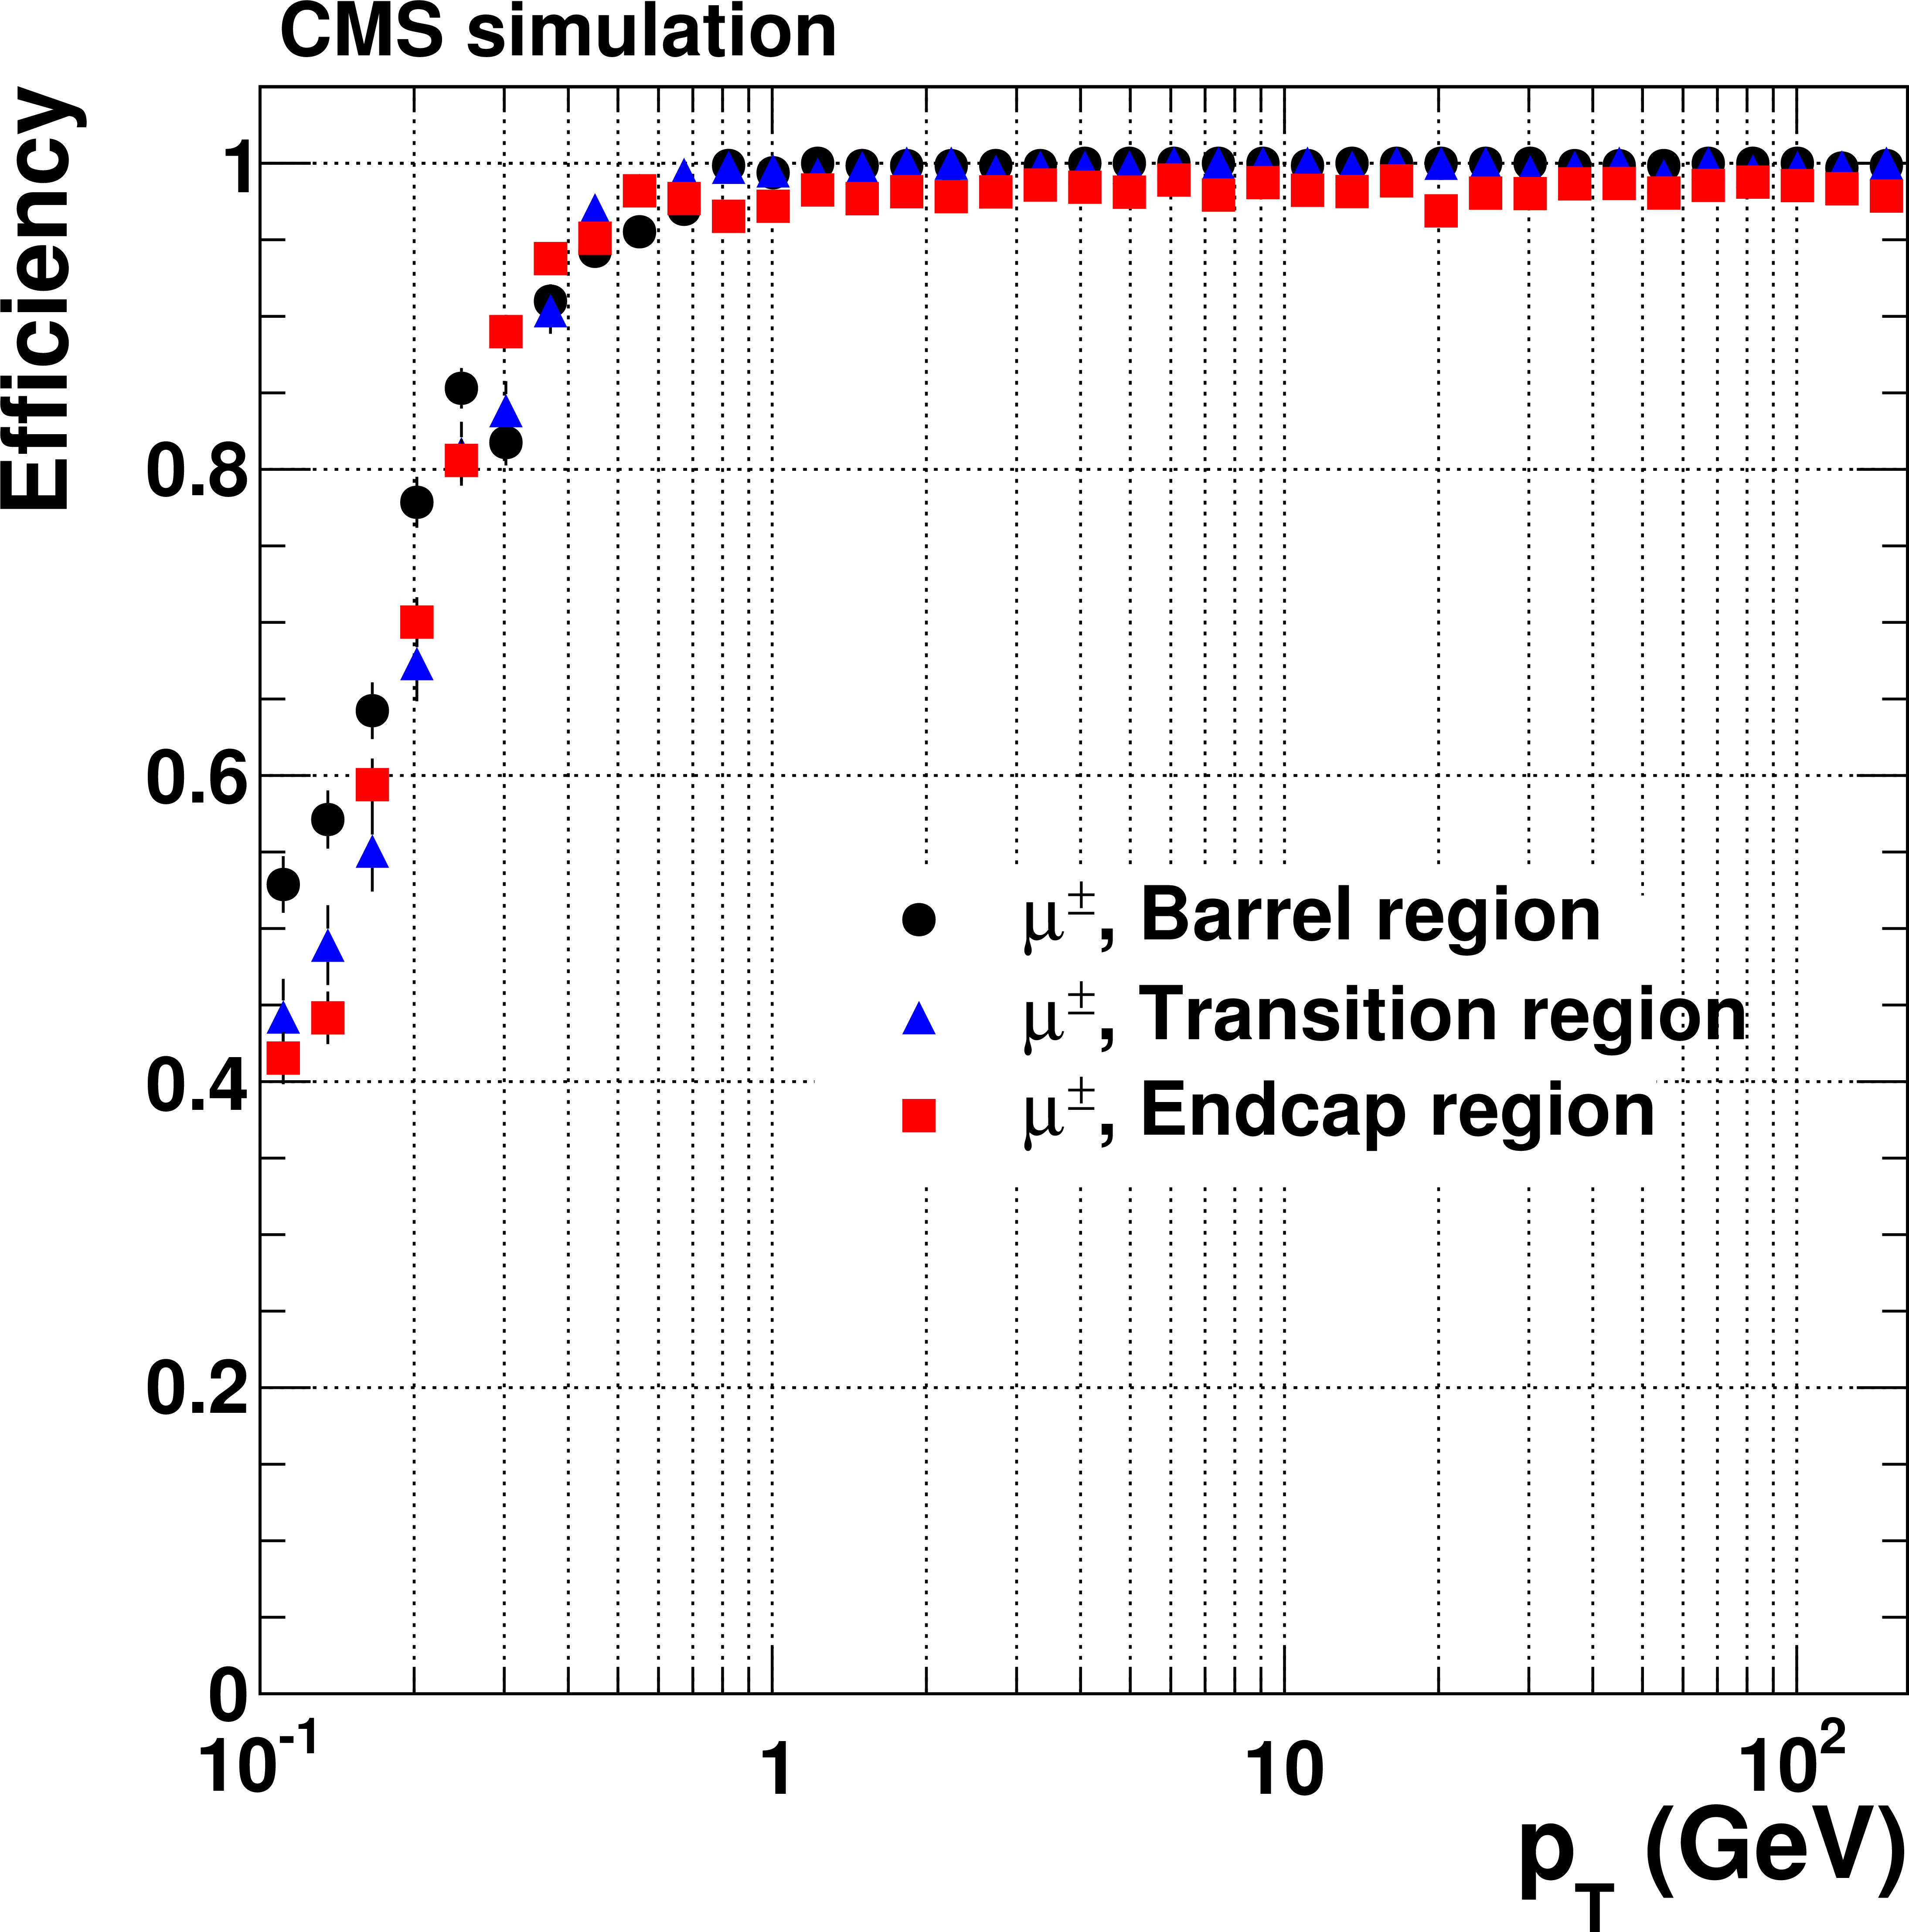
\includegraphics[width=0.35\textwidth]{figuras/Chapter3/TrackEff_Muon_pt.png}
    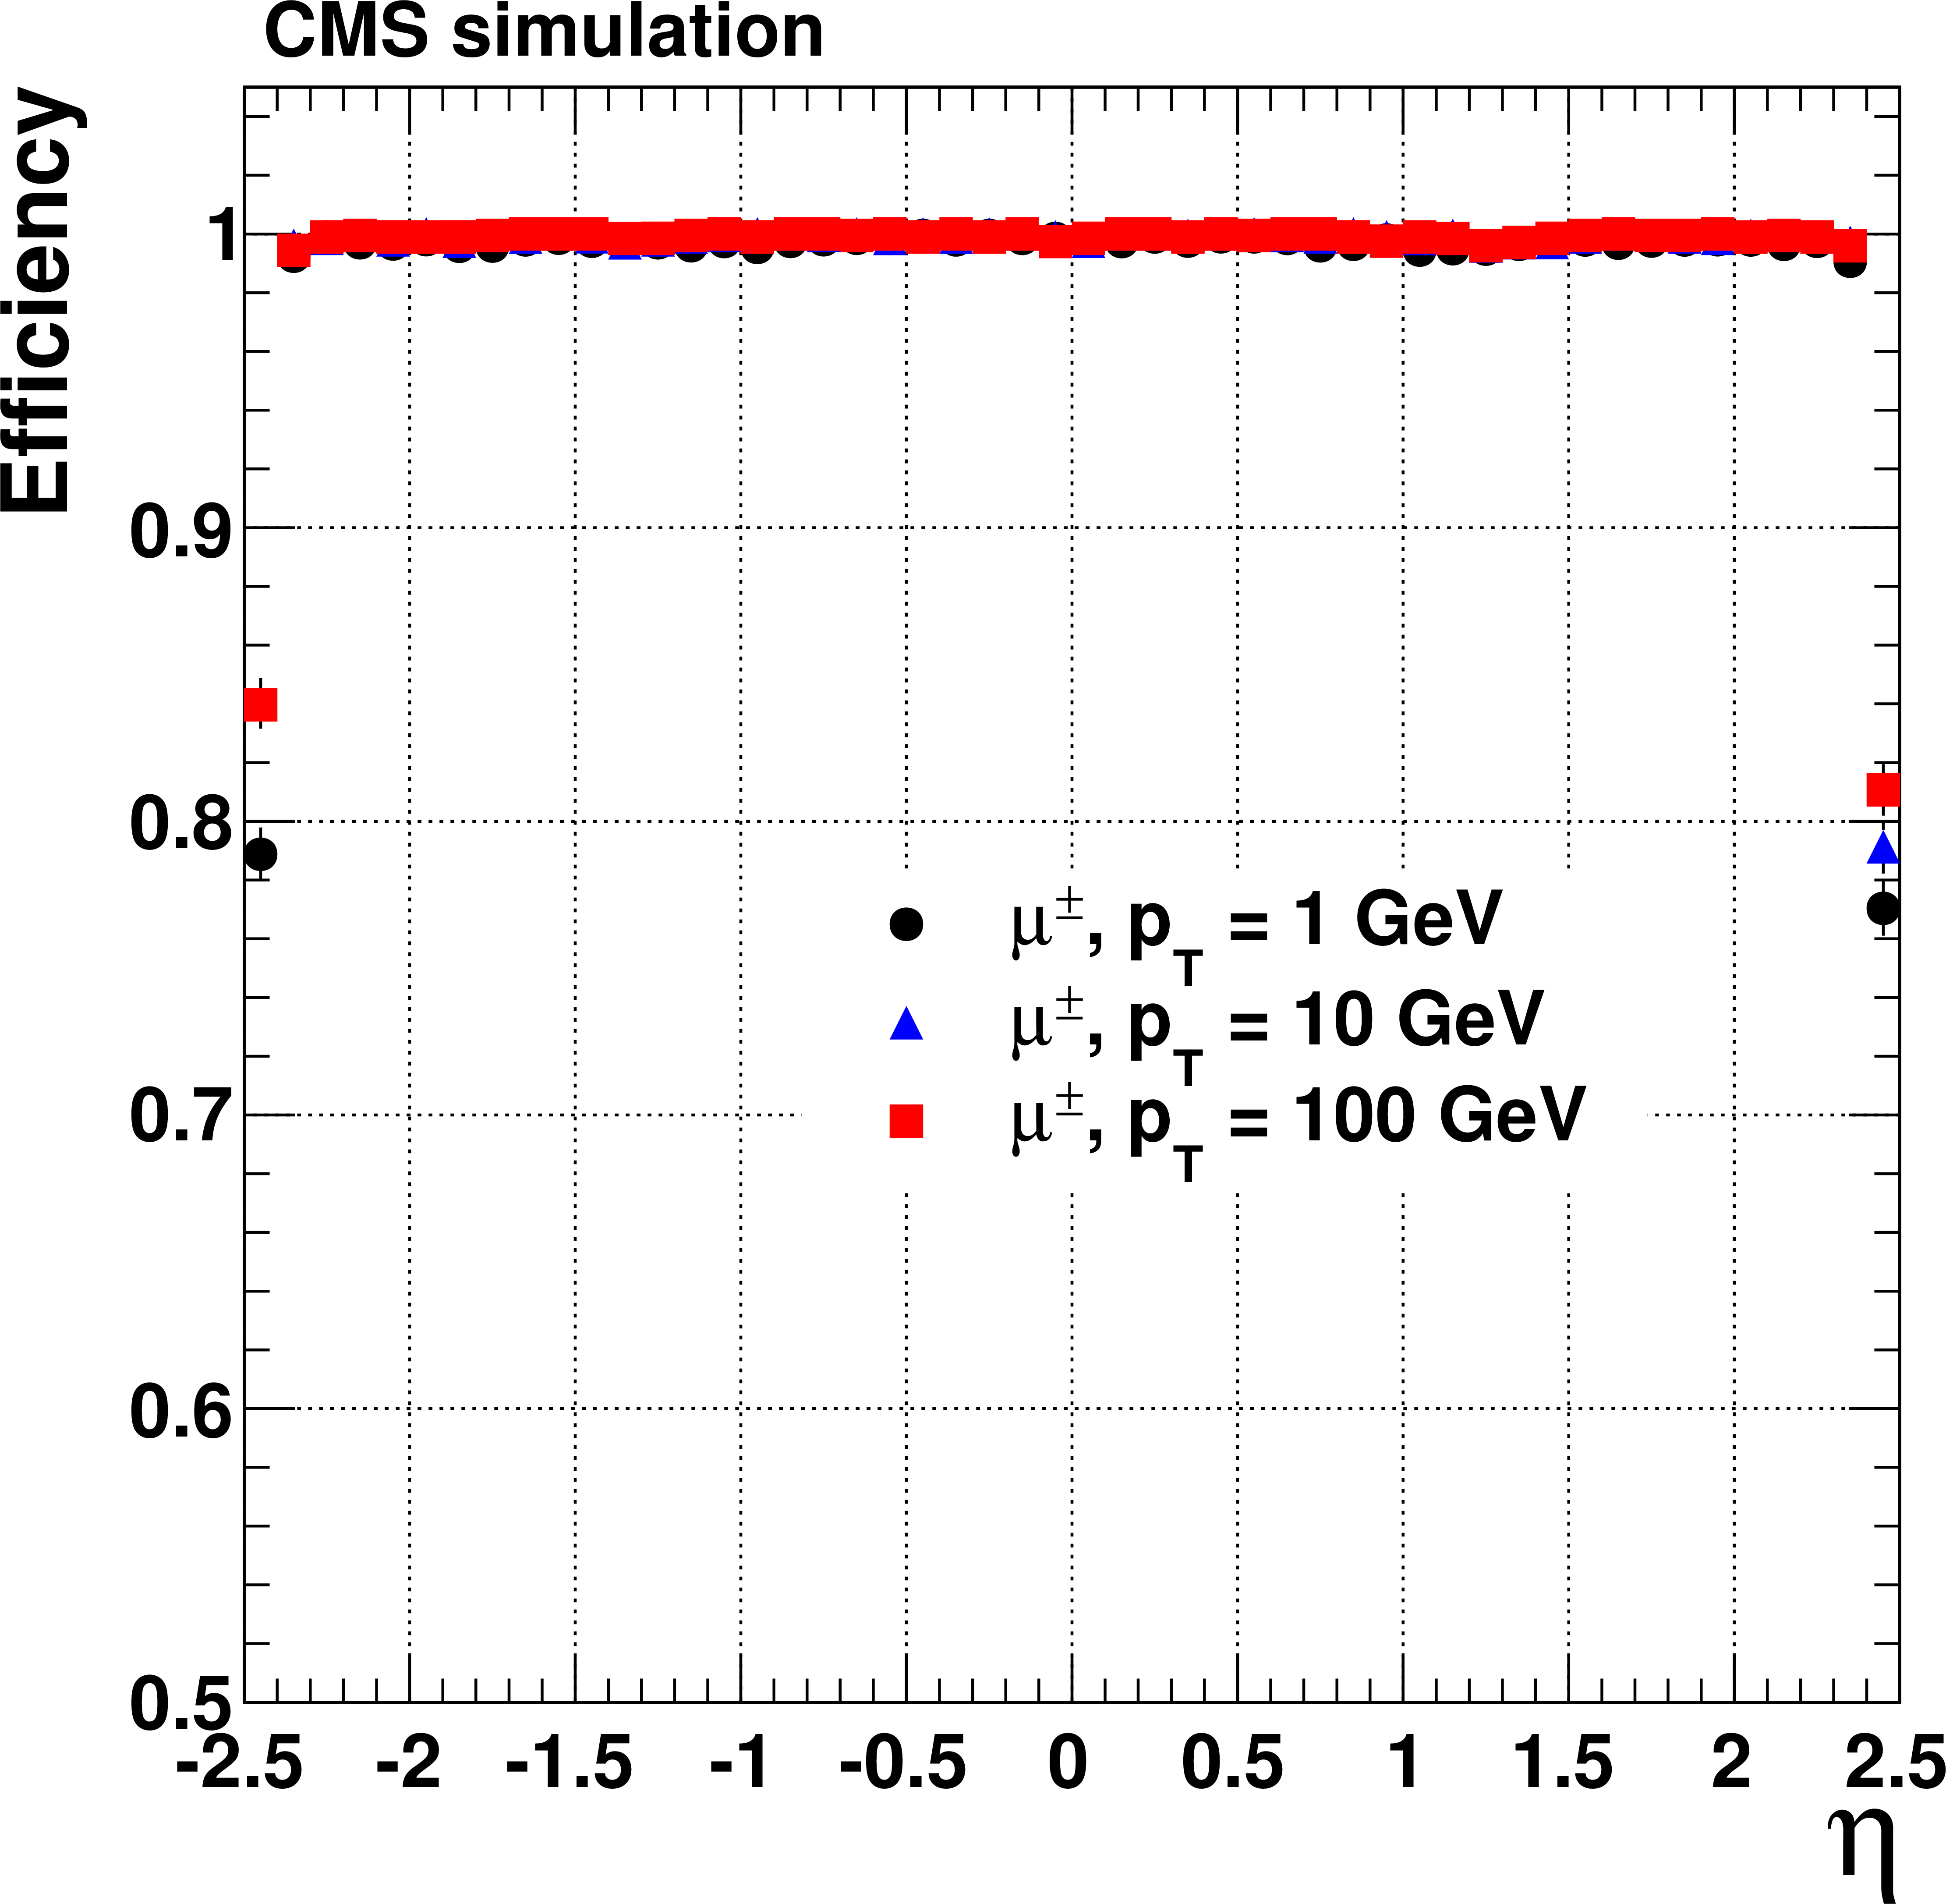
\includegraphics[width=0.35\textwidth]{figuras/Chapter3/TrackEff_Muon_eta.png}
    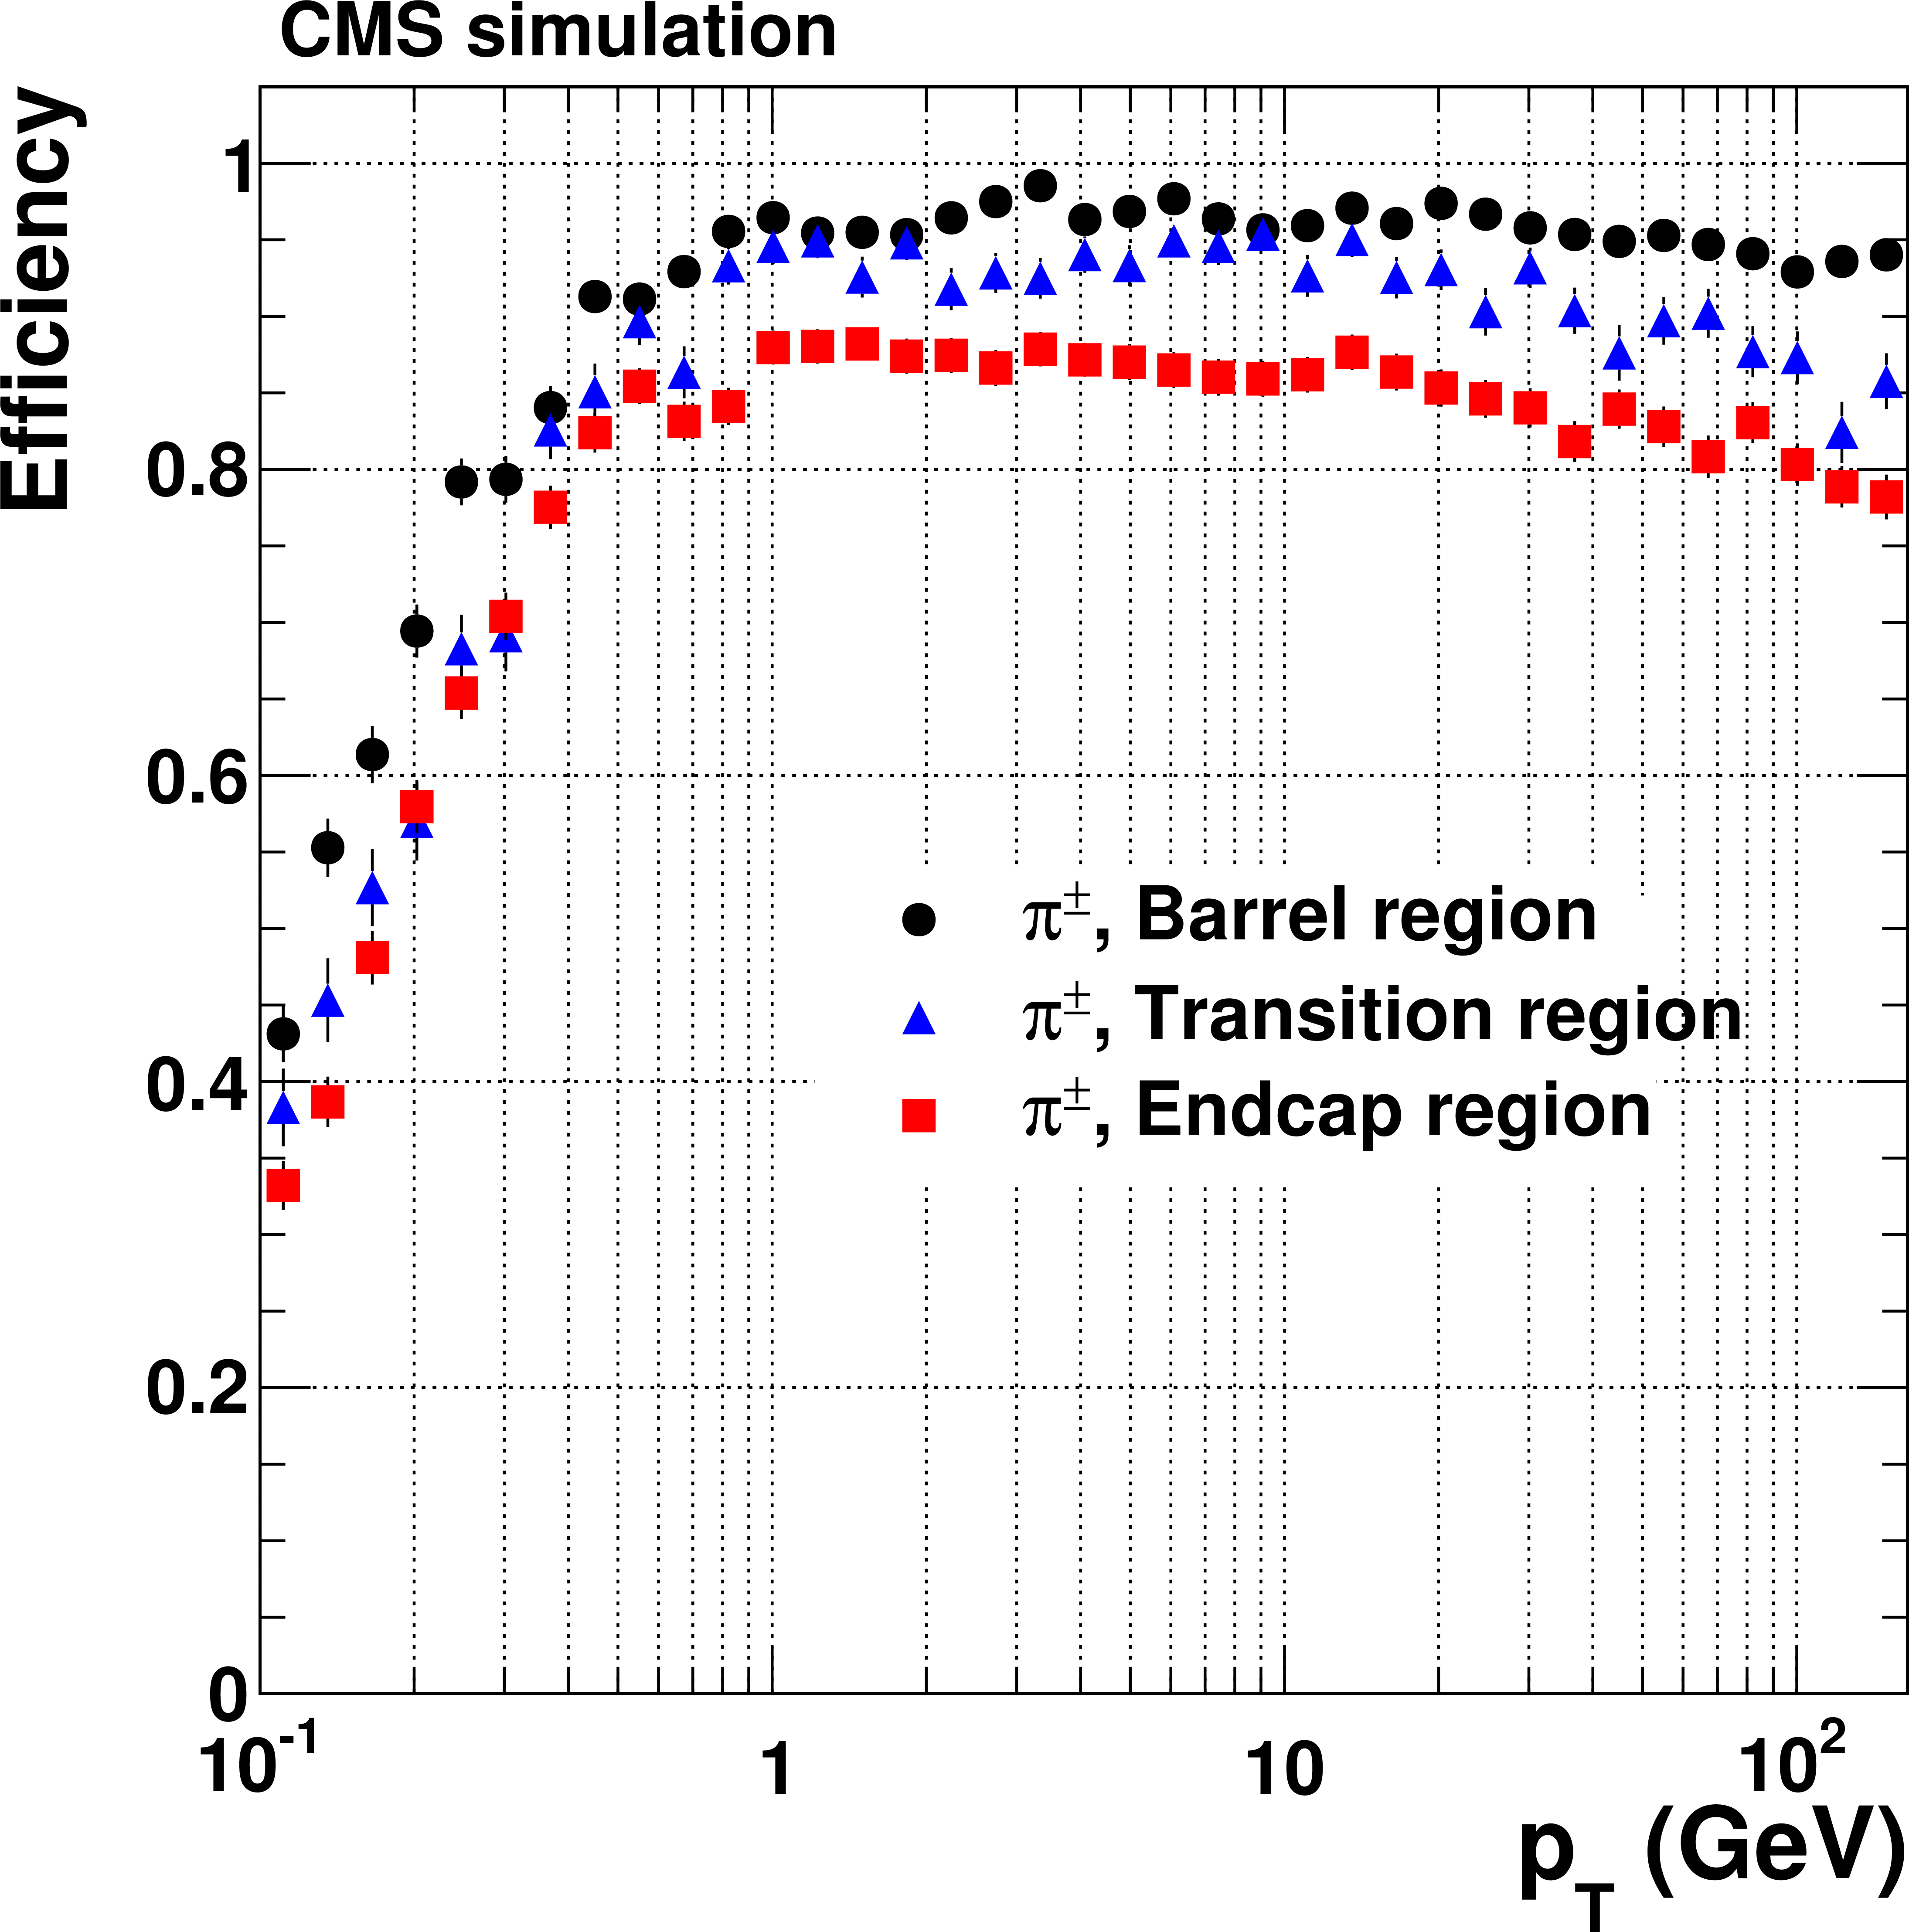
\includegraphics[width=0.35\textwidth]{figuras/Chapter3/TrackEff_Pion_pt.png}
    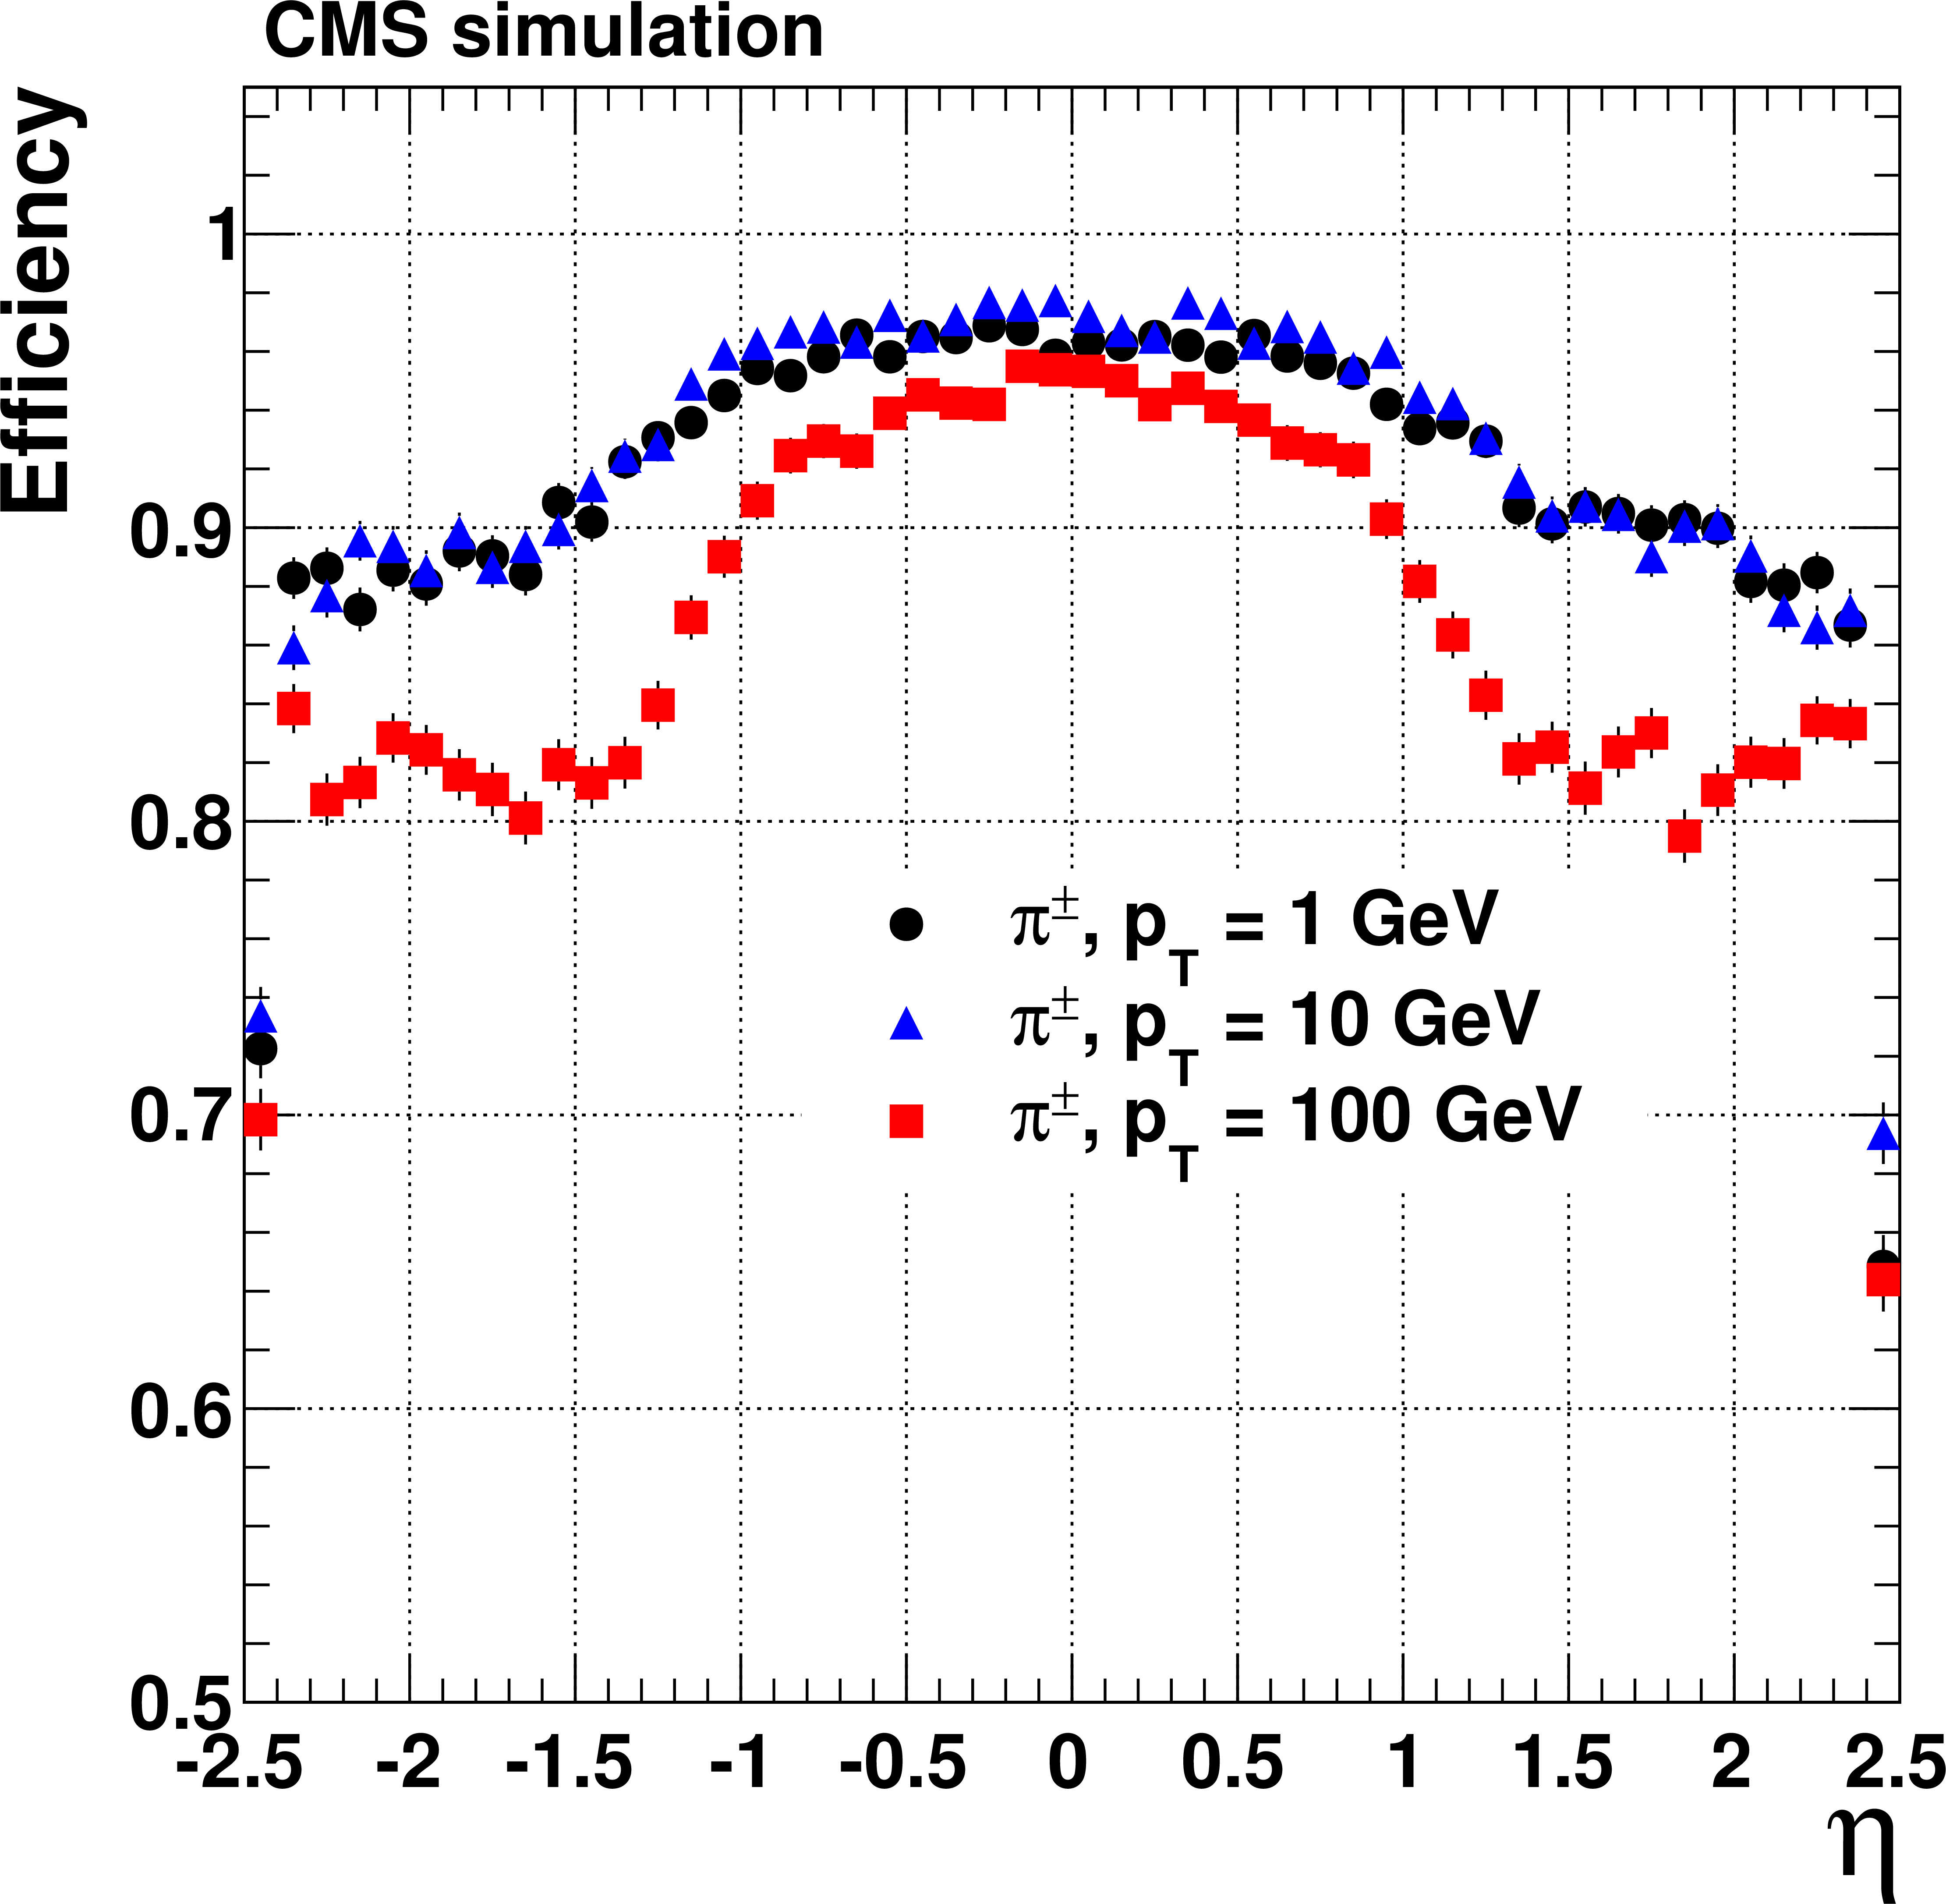
\includegraphics[width=0.35\textwidth]{figuras/Chapter3/TrackEff_Pion_eta.png}
    \caption{Efficiency of reconstructed track as function of $p_{\textrm{T}}$ and $\eta$ for 
    muons (top) and charged pions (bottom). Efficiencies were obtained using pp collisions with a centre-of-mass 
    energy of $\sqrt{s} =$  7 TeV, which corresponds to 2011 data. For simulated data an average of 8 pileup 
    events was used, which is roughly the amount delivered by the LHC on 2011. Figure taken from \cite{Chatrchyan:2014fea}}
    \label{fig:Track_Efficiencies}
  \end{center}
\end{figure}

\subsection{Vertex Reconstruction}

%Primary vertex reconstruction is performed with the purpose to measure the position, and the uncertainty, 
%of all vertices produced in the pp collisions, such as the vertex produced by a hard interaction, secondary 
%vertices coming from b-jets as well as pileup collisions. Vertex reconstruction first proceed with a 
%track selection, then reconstructed tracks are clustered to identify vertices, and finally the vertex position
%is determined by a fit. \\

Primary vertex reconstruction is performed with the purpose to measure the position, and the uncertainty, 
of all vertices produced in the pp collisions. Vertex reconstruction first proceed with a 
track selection, then reconstructed tracks are clustered to identify vertices, and finally the vertex position
is determined by a fit. The main criteria for track selection are the impact parameter relative to the beam spot, the
number of reconstructed hits in the tracker and the $\chi^{2}$ associated to its trajectory. Then, the 
selected tracks are grouped into clusters according to its z-coordinate with the aim of identifying
all possible vertices even for inelastic collisions. Track clustering is performed with the 
deterministic annealing (DA) algorithm \cite{VertexRecoBIB}. The DA algorithm resolves iteratively
the z-coordinates of all the possible vertices and the cluster of tracks associated to them, in a similar way 
to solve a physical system with many degrees of freedom, approaching iteratively to the state 
of minimum energy \cite{Chatrchyan:2014fea}. Finally, the adaptive vertex fitter technique \cite{Frühwirth:1027031}
is used in order to perform the best estimation of the vertex parameters, in particular the position,
from fitting the cluster of tracks associated to the vertex. The primary vertex is selected from the vertex with the higher
sum of $\textrm{p}_{\textrm{T}}^{2}$ of the cluster of tracks.\\

The resolution of the primary vertex depends on the number of tracks associated to it. Figure \ref{fig:RecoVertex} 
shows the resolution of x and z position for primary vertex reconstruction, using minimum vias samples 
\footnote{minimum vias samples pass a suit of triggers and minimum requirements on hit 
or track multiplicity} and jet-enriched data samples \cite{Chatrchyan:2014fea}. The resolution for x and z position 
is, respectively, less than 20 $\mu$m and 25 $\mu$m for the minimum vias samples while it is 
improved to less than 10 $\mu$m and 12 $\mu$m for jet-enriched samples. Figure \ref{fig:RecoVertex} c) shows
the efficiency of primary-vertex reconstruction which depends on the number of tracks. 

\begin{figure}[ht]
  \begin{center}
    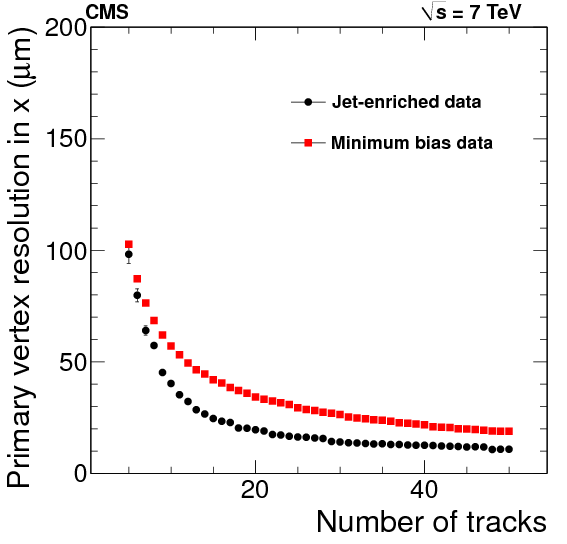
\includegraphics[width=0.3\textwidth]{figuras/Chapter3/RecoVertex_x_resolution.png}
    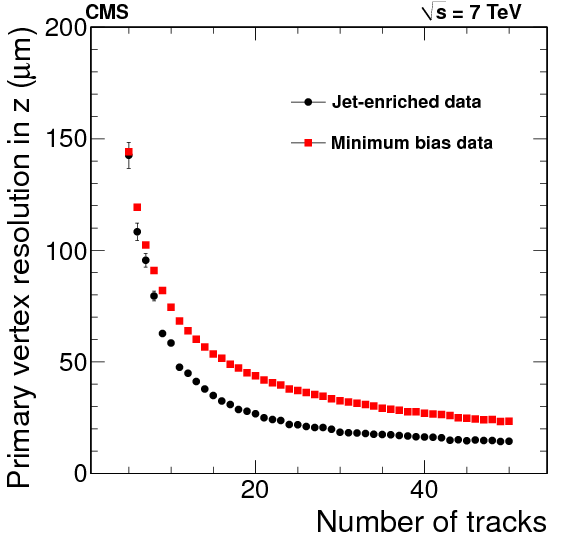
\includegraphics[width=0.3\textwidth]{figuras/Chapter3/RecoVertex_y_resolution.png}
    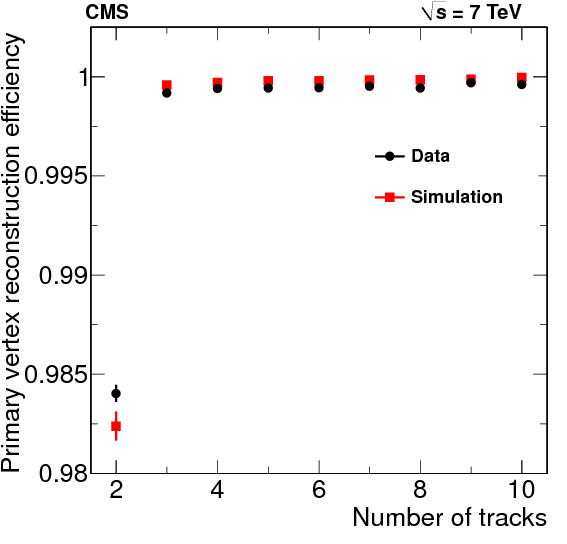
\includegraphics[width=0.3\textwidth]{figuras/Chapter3/Effciiency_vertex_resolution.png}
    \caption{Resolution of x and z position  for primary vertex reconstruction, using a) minimum vias samples and b) jet-enriched samples. 
    Resolution is improved using jet-enriched samples since in these sample the mean of $\textrm{p}_{\textrm{T}}$ is larger than minimum vias samples.  
    For efficiency of primary vertex reconstruction shown in c), minimum vias MC samples were used. Results were estimated 
    with pp collisions with a centre-of-mass energy of $\sqrt{s} =$  7 TeV. Figures were taken from \cite{Chatrchyan:2014fea}.}
    \label{fig:RecoVertex}
  \end{center}
\end{figure}

%El algoritmo lo que hace es buscar la minima temperatura ``T'' local para el cual chi2 sea minima, 
% comienza con T-> inf, todos los tracks estan asociados a un solo vertice, la T comienza a disminuir,
% comienza a crecer el numero de vertices, se hace eso hasta que el sistema alcanza la Tcritica (el punto de inflexion de la energia libre F)
% (chi2 hace las veces de la eneria)
% una vez se encuentra el minimo local, cada vertice se convierte en dos, endonde el peso asociados a esos vertices es igual al vertice ``papa''
% eso se hace iterativamente hasta alcanzar una T igual a 4 en donde ya hay una posibilidad de convertir un real vertice en dos.


\subsection{Clustering}
\label{subsec:Clustering}
Other important part of the PF technique, in addition to the tracks, is the reconstruction of the 
calorimetric clusters. The calorimeter clusters are used to identify the energy deposits which come from 
%neutral-visible particles, such as photons and neutral hadrons, and discriminate them from the energy deposits 
photons and neutral hadrons, and to discriminate them from the energy deposits due charged hadrons; 
besides it reconstructs the electrons along with their associated Bremsstrahlung radiation
and helps to determinate the track parameters of the charged hadrons which were not measured 
accurately from the track reconstruction (for example, charged hadrons that are outside of the tracker acceptance, or 
charged hadrons with high $p_{\textrm{T}}$). The clustering is performed for 
each part of the CMS calorimeter system: ECAL, HCAL, HF and PS.\\

The clustering algorithm proceeds from the ``cluster seeds'' identified at local level. Cluster seeds are selected 
from individual calorimeter cells which have a maximal energy deposits above a given energy. Once the cluster seed is selected,
the algorithm searches for energy deposits in the  boundary cells with a common side. The algorithm aggregates to the cluster 
at least one additional cell with a maximum energy higher than two standard deviations from the electronic noise: for the ECAL, 80 $\textrm{MeV}$ in 
barrel and up to 300 $\textrm{MeV}$ in the end-caps for the ECAL, while 800 $\textrm{MeV}$ for the HCAL \cite{CMS-PAS-PFT-09-001}. This
cells combined are known as ``topological clusters''. The topological clusters are taken as ``particle flow clusters'' seeds
in order to solve any overlapping among clusters.

\subsection{Link algorithm}
\label{subsec:Linkalgorithm}
As mentioned earlier, a particle is expected to produce signatures in different sub-detectors, giving rise to one or more 
so-called PF elements: tracks, clusters and tracks in the muon system; for example, 
a charged hadron as the pion, would produce a track in the inner tracker along with 
energy deposits in both calorimeters. PF uses the \textit{link algorithm} to perform a topological combination 
of the PF elements reconstructed in the different sub-detectors with the aim of reconstructing fully each particle in the event. \\
%of the PF elements recontructed in the different subdetectors with the aim of identifying the type of each particle in the event. 

The link between a charged particle track and a calorimeter cluster is performed as follows:

\begin{itemize}
 \item The track is extrapolated from the last hit reconstructed in the tracker to: the two layers in the PS, the expected depth
 for an electron shower in the ECAL and one interaction length for an typical hadron shower in the HCAL. 
 \item The track is linked to a cluster if the extrapolated position in the calorimeter is within the cluster boundaries. 
 \item The distance in the $\eta-\phi$ plane between the extrapolated track position and the cluster position defines the quality of the link. 
\end{itemize}

Similarly, two calorimeter clusters (i.e. links between PS and ECAL clusters or links between ECAL and HCAL clusters) are linked when the 
extrapolated position in the more granular calorimeter (PS or ECAL) is within 
the boundaries of the less granular calorimeter (ECAL or HCAL). For example, the link between the ECAL and HCAL clusters
produced by a pion is established when the extrapolated position from the ECAL is within the HCAL cluster boundary. Finally, the 
link between a charged particle track reconstructed in the tracker and a track in the muon system (known as global muon) 
is established by a global fit between the two tracks and its $\chi^{2}$ defines the quality of the link.  

\section{Jets Reconstruction}
\label{sec:Jet}


% Jets are reconstructed with the Particle Flow technique (PF) using the anti$-$k$_{T}$ algorithm \cite{Alwall:2011uj}.
The PF technique \cite{CMS-PAS-PFT-09-001} takes the information collected by the CMS sub-detectors in order to identify and reconstruct
all the visible final-state particles (electrons, muons, photons, charged hadrons and neutral hadrons) produced
in the hard interaction. The PF technique reconstructs the jet constituents individually from the
combination of tracks and calorimeter clusters. Then, the jet reconstruction is performed
with the anti$-$k$_{T}$ algorithm \cite{AntiKTAlgorithm} iterating over all the PF objects, using a distance parameter of
$\Delta R = 0.4$ in the $\eta-\phi$ plane, where $\Delta R = \sqrt{(\Delta \phi)^2+(\Delta \eta)^2}$.\\

\begin{figure}[ht]%[!Hhtbp]
  \begin{center}
    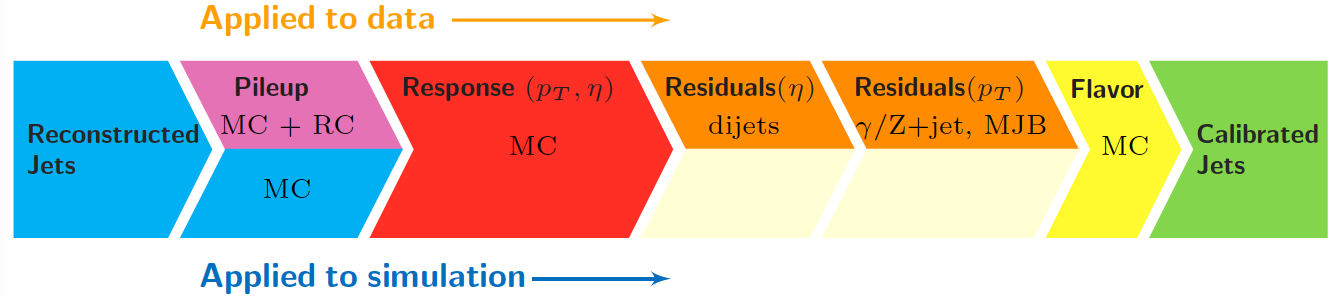
\includegraphics[width=0.9\textwidth]{figuras/Chapter3/JEC_levels.png}
    \caption{Levels of corrections for PF jet four-momentum. Figure taken from \cite{JESandJER}}
    \label{fig:JEC_levels}
  \end{center}
\end{figure}

The four-momentum of the reconstructed jet is the addition of the four-momenta of all the PF objects associated to the jet. However
due to detector responses and experimental effects, the PF jet four-momentum does not correspond to the four-momentum
at parton or hadron level; therefore, jet energy corrections (JEC) are required. Figure \ref{fig:JEC_levels} shows the different
levels of corrections which are applied in a fixed sequence. Each correction corresponds to a multiplicative factor $C$ on
the PF jet four-momentum ($p_{\mu}^{raw}$):

\begin{equation}
 p_{\mu}^{corrected} = C \times p_{\mu}^{raw}
\end{equation}

The first step in the chain is the ``L1 corrections'' (also referred as ``pileup offset''). It corrects the additional tracks and the excess of energy deposits
in the calorimeters due pile-up events . The amount of the pile-up contribution
to the jet energy can be estimated from the global per-event $p_{T,offset}$ density $\rho$ and the jet area \cite{JECpileup}. This amount
is obtained from simulated dijet events with and without PU. \\

The second level of JEC is related to the detector response to hadrons (L2L3 MC-truth corrections), correcting
the non-uniformity in $\eta$ and the non-linearity in $p_{T}$. The simulated jet response is determined
with QCD-multijet events generated with Pythia and with a simulation of the CMS detector based
on Geant4.\\

After these steps, the L2L3 Residual corrections are applied in order to address the remaining difference
between the jet response on data and MC (of the order of $1 \%$). This corrections are achieved with data-driven methods, using
dijet samples for $\eta$-dependent corrections and $\gamma /$Z+jets samples for the corrections to $p_{T}$. The last stage
of the JEC (L5) is optional and it accounts the jet-flavor corrections. \\

%An efficiency larger than 80% is obtained for jets with a p T > 20 GeV/c. The 100% plateau is reached above
%40 GeV/c, at which point the mismatched jet rate is negligible





%JER Article
%The jet p T resolutions are determined with both dijet and photon+jet events, as discussed in
%section 8. The reference resolutions obtained from simulation are parameterized as a function of
%particle-level jet p T, ptcl (defined in section 2) and average number μ of pileup interactions in bins
%of jet η. Corrections for differences between data and MC simulation are applied as η-binned scale
%factors




%Since in average 85 $\%$ of the constituents of a jet are charged particles and photons, the jet energy resolution

%PF jet momentum and spatial resolutions are greatly improved with respect to calorimeter jets, as
%the use of the tracking detectors and high granularity of the ECAL improves the energy resolution
%through the independent measurements of charged hadrons and photons inside a jet, which together
%2.1constitute ≈85% of the average jet energy. In reconstructing the PF candidate four-momentum,
%photons are assumed massless and charged hadrons are assigned the charged pion mass.

%As mentioned previously, the typical jet energy fractions carried by charged particles, photons
%and neutral hadrons are 65%, 25% and 10% respectively. These fractions ensure that 90% of
%the jet energy can be reconstructed with good precision by the particle-flow algorithm, both in
%value and direction, while only 10% of the energy is affected by the poor hadron calorimeter
%resolution and by calibration corrections of the order of 10 to 20%. As a natural consequence,
%it is expected that jets made of reconstructed particles be much closer to jets made of MonteCarlo–generated
%particles than jets made from the sole calorimeter information, in energy, direction
%and content. It is the purpose of this section to quantify this statement.

%($c\tau > 1$ cm)


%\subsection{Online Identification}
%\label{subsec:JetTrigger}

%\subsection{Offline Identification}
%\label{subsec:JetReconstruction}



%\subsection{Online Identification}
%\label{subsec:ElectronTrigger}

%\subsection{Offline Identification}
%\label{subsec:ElectronReconstruction}
\section{MET}
\label{sec:MET}

\section{Photon Reconstruction}
\label{sec:Photon}


\section{Muon Reconstruction}
\label{sec:Muon}

\section{Electron Reconstruction}
\label{sec:Electron}

\section{B-Jet Reconstruction}
\label{sec:BJet}



\section{Tau Lepton}
\label{sec:Tau}

%\subsection{Tau Reconstruction}
%\label{subsec:TauTrigger}

\subsection{Tau Reconstruction}
\label{subsec:TauReconstruction}

\subsection{Working Points}
\label{subsec:wp}

\subsubsection{Efficiency of Working Points}
\label{subsubsec:Eff_WP}

\subsection{Fake Rates}
\label{subsec:FakeRates}

\subsection{Perspectives Run III}
\label{subsec:Perspectives} 